\documentclass[11pt]{article}

\usepackage[margin=1in]{geometry}
\usepackage{amsmath, amssymb}
\usepackage{graphicx}
\usepackage{booktabs}
\usepackage{hyperref}
\usepackage{caption}
\usepackage{subcaption}
\usepackage{tikz}
\usetikzlibrary{arrows.meta, positioning, calc}

\title{How do transformers learn Hidden Markov Models?\\
       A case study on the cylinder graph HMM\@.}
\date{\today}

\begin{document}
\maketitle

%----------------------------------------------------------------------
\section{Introduction}\label{sec:intro}
%----------------------------------------------------------------------

Next-token prediction---the task of estimating $P(X_{t+1} \mid X_{\le t})$---is the training objective underlying modern large language models (LLMs).  Trained on this objective alone, LLMs develop rich internal representations---grammar, factual knowledge, reasoning patterns---none of which were explicitly programmed.  A natural scientific question is: \emph{what computational structure does the model build internally in order to make good predictions?}

To understand what transformers learn, a line of recent work has turned to synthetic datasets for which ground truth is known analytically.  In this report we consider Hidden Markov Models (HMMs) as the data-generating process.  An HMM is a two-layer stochastic process.  A hidden (unobserved) variable $Z_t$ evolves as a Markov chain on a finite state space of size~$N$, with transition matrix $A_{ij} = P(Z_{t+1}{=}j \mid Z_t{=}i)$.  At each time step, the current hidden state emits an observable token $X_t$ from a vocabulary of size~$K$, with probabilities $B_i(\mu) = P(X_t{=}\mu \mid Z_t{=}i)$.  The observer sees only the token sequence $X_1, X_2, \ldots$, but the hidden states remain hidden.  Although the hidden process is Markovian, the observed token sequence is \emph{not}: the marginal process $\{X_t\}$ exhibits autocorrelations that encode the latent dynamics.

A \textbf{transformer} takes as input a sequence of discrete tokens and outputs, at each position, a conditional probability distribution over the next token---it is an autoregressive model.  The first layer is an \emph{embedding}: each token is mapped to a continuous vector in $\mathbb{R}^d$.  This embedding serves as a learned compression of the discrete vocabulary into a geometry where semantically related tokens lie nearby---a phenomenon famously illustrated by the discovery of meaningful directions in word-embedding spaces (e.g.\ ``king'' $-$ ``man'' $+$ ``woman'' $\approx$ ``queen'').  The embedding vectors are then processed by a stack of layers (self-attention and optional feedforward sublayers) that mix information across positions, and a final linear projection followed by a softmax produces the predicted next-token distribution $\hat{P}(X_{t+1} \mid X_{\le t})$.  A transformer with \emph{context window} of length~$T$ can condition on at most $T$ preceding tokens.

An HMM is a particularly natural test case because the forward algorithm allows us to compute $P(X_{1:T} \mid \lambda)$ exactly for any observation sequence.  Moreover, the algorithm yields the \emph{belief state}---the posterior distribution over hidden states given the observations so far---which is a sufficient statistic for next-token prediction and can be viewed as the analogue of an ``internal world model'' in the context of LLMs.  The entropy rate of the process sets an absolute lower bound on the prediction loss, and the Bayes-optimal loss at finite context provides a tighter bound for models that can only look back a fixed number of steps.

We seek to answer the following questions about how transformers learn to model HMMs:
\begin{enumerate}
  \item \textbf{How close can a transformer get to the information-theoretic optimum?}  By comparing the trained model's loss against the entropy rate and the Bayes-optimal loss, we can cleanly decompose the gap into a \emph{finite-context cost} (inherent to the architecture's limited memory) and a \emph{capacity gap} (how far the model's learned strategy is from optimal given its context window).
  \item \textbf{What internal representations does the model learn?}  If the forward algorithm is the optimal computation, does the transformer discover something analogous to belief states?  We can inspect the model's learned embeddings and intermediate activations to look for signatures of the latent HMM structure.
\end{enumerate}

We study these questions on a specific HMM called the ``cylinder graph HMM'' (Section~\ref{sec:hmm}).  The key findings are:
\begin{itemize}
  \item The best transformer (206k parameters) reaches within ${\sim}0.004$~nats of the Bayes-optimal predictor at its context length, meaning it has essentially learned to perform near-optimal Bayesian filtering.
  \item Transformers consistently outperform $n$-gram models, which memorise token co-occurrence statistics, suggesting they learn something qualitatively beyond counting.
  \item The learned token embeddings spontaneously discover the depth-level structure of the HMM---tokens from the same hidden-state cluster are mapped to similar directions in embedding space---without any supervision about this structure.
\end{itemize}

The remainder of this report is organised as follows.  Section~\ref{sec:prelim} introduces the mathematical background on HMMs, belief states, and transformers.  Section~\ref{sec:hmm} defines the cylinder graph HMM\@.  Section~\ref{sec:baselines} derives the information-theoretic baselines.  Section~\ref{sec:transformers} describes the transformer architectures and training procedure.  Section~\ref{sec:results} presents results on scaling, architecture, and embedding structure.  Section~\ref{sec:summary} concludes with open questions.

%----------------------------------------------------------------------
\section{Technical Preliminaries}\label{sec:prelim}
%----------------------------------------------------------------------

\subsection{Hidden Markov Models}\label{sec:hmm-def}

A Hidden Markov Model~\cite{baum1966,rabiner1986,rabiner1989} is a doubly stochastic process consisting of an underlying Markov chain whose states are not directly observable, coupled with state-dependent observation distributions that produce the data we observe.  Formally:
\begin{itemize}
  \item \textbf{State space.}  The hidden state $Z_t$ takes values in a finite set $S$ with $|S| = N$.
  \item \textbf{Observations.}  The observable token $X_t$ takes values in a finite set $\Omega$ with $|\Omega| = K$.
  \item \textbf{Markov assumption.}  $P(Z_t \mid Z_{<t}) = P(Z_t \mid Z_{t-1})$.
  \item \textbf{Observation independence.}  $P(X_t \mid Z_t, Z_{<t}) = P(X_t \mid Z_t)$.
\end{itemize}

The model is parameterised by the triple $\lambda = (A, B, \pi)$:
\begin{align}
  A_{ij}    &= P(Z_{t+1}{=}j \mid Z_t{=}i),     &\text{(transition matrix)} \\
  B_i(\mu)  &= P(X_t{=}\mu \mid Z_t{=}i),        &\text{(emission probabilities)} \\
  \pi_i     &= P(Z_1{=}i).                        &\text{(initial distribution)}
\end{align}
Note that while the hidden states are Markovian, the marginal process over observations is \emph{not}.

As a concrete example, consider the Z1R process~\cite{rabiner1989}: a three-state HMM with two observable tokens.  State $A$ deterministically emits ``0'' and transitions to $B$; state $B$ deterministically emits ``1'' and transitions to $C$; state $C$ emits a fair coin flip (``0'' or ``1'') and always returns to $A$.  The observed sequence therefore has the pattern $0, 1, \text{(random)}, 0, 1, \text{(random)}, \ldots$ --- a period-3 structure masked by the coin flip.  Although each state transitions deterministically, an observer who sees only the tokens cannot distinguish whether a ``0'' came from state $A$ or from the coin flip in state $C$.  This simple example already illustrates the core challenge: optimal prediction requires tracking a \emph{distribution} over hidden states, not just the most recent tokens.

The joint probability of a state sequence $Z_{1:T}$ and observation sequence $X_{1:T}$ factorises as
\begin{equation}\label{eq:joint}
  P(X_{1:T}, Z_{1:T} \mid \lambda)
  = \pi_{Z_1}\, B_{Z_1}(X_1) \prod_{t=2}^{T}
    A_{Z_{t-1},Z_t}\, B_{Z_t}(X_t).
\end{equation}

Rabiner~\cite{rabiner1989} organised HMM computation into three canonical problems:

\begin{center}
\begin{tabular}{llll}
  \toprule
  Problem & Given & Compute & Algorithm \\
  \midrule
  \textbf{Evaluation} & $\lambda$, $X_{1:T}$ & $P(X_{1:T} \mid \lambda)$
    & Forward algorithm \\
  \textbf{Decoding} & $\lambda$, $X_{1:T}$
    & $\arg\max_{Z_{1:T}} P(Z_{1:T} \mid X_{1:T}, \lambda)$
    & Viterbi algorithm \\
  \textbf{Learning} & $X_{1:T}$
    & $\arg\max_{\lambda} P(X_{1:T} \mid \lambda)$
    & Baum--Welch (EM) \\
  \bottomrule
\end{tabular}
\end{center}

\noindent In this paper we are concerned exclusively with the \emph{evaluation} problem: the HMM parameters are known by construction, so neither Viterbi decoding nor Baum--Welch re-estimation is needed.

\subsection{The Forward Algorithm}\label{sec:forward}

The evaluation problem asks: given $\lambda$ and $X_{1:T}$, what is $P(X_{1:T} \mid \lambda)$?  A na\"ive marginalisation over all hidden state sequences requires summing $N^T$ terms.  The key observation is that the joint probability~\eqref{eq:joint} has a sequential structure: the contribution of each time step depends only on the previous hidden state.  This allows us to accumulate the sum inductively---processing one time step at a time and carrying forward an $N$-dimensional vector that summarises all paths so far.  This is the forward algorithm, which reduces the cost from $O(N^T)$ to $O(N^2 T)$.

Define the \emph{forward variable} $\alpha_t(j) := P(X_{1:t},\, Z_t{=}j \mid \lambda)$---the joint probability of observing $X_{1:t}$ and being in state~$j$ at time~$t$.

\paragraph{Initialisation ($t=1$):}
\begin{equation}
  \alpha_1(j) = \pi_j\, B_j(X_1), \qquad j = 1,\ldots,N.
\end{equation}

\paragraph{Recursion ($t = 1,\ldots,T{-}1$):}
\begin{equation}\label{eq:forward-recursion}
  \alpha_{t+1}(j)
  = \biggl[\sum_{i=1}^{N} \alpha_t(i)\, A_{ij}\biggr] B_j(X_{t+1}).
\end{equation}

\paragraph{Termination:}
\begin{equation}
  P(X_{1:T} \mid \lambda) = \sum_{j=1}^{N} \alpha_T(j).
\end{equation}

In matrix--vector form, writing $\boldsymbol{\alpha}_t$ as a row vector and $D_t = \mathrm{diag}(B_1(X_t),\ldots,B_N(X_t))$:
\begin{equation}\label{eq:forward-matrix}
  \boldsymbol{\alpha}_T
  = \boldsymbol{\pi}^\top D_1\, A\, D_2\, A\, D_3
    \cdots A\, D_T.
\end{equation}
The complexity is $O(N^2 T)$ in time and $O(N)$ in space when only the final likelihood is needed.  For long sequences, $\alpha_t(j)$ underflows exponentially; standard remedies include log-space computation (log-sum-exp trick) or Rabiner's scaling coefficients.

\subsection{Belief States and Optimal Prediction}\label{sec:belief}

Define the \emph{belief state}
\begin{equation}\label{eq:belief-def}
  \eta_t(j)
  := P(Z_t{=}j \mid X_{1:t})
  = \frac{\alpha_t(j)}{\sum_{l=1}^{N} \alpha_t(l)},
\end{equation}
the posterior distribution over hidden states given the observations so far.  Note the structural parallel with the transfer-matrix formalism in statistical mechanics: the forward variable $\boldsymbol{\alpha}_t$ is propagated by a product of observation-dependent matrices $A\,D_t$ (Eq.~\ref{eq:forward-matrix}), and the belief state is its normalised version, much as the dominant eigenvector of a transfer matrix encodes equilibrium probabilities.

The belief state obeys a recursive update.  Define the \emph{symbol-labelled transition matrix} $T^{(x)}_{ij} = A_{ij}\, B_j(x)$, which combines transition and emission into a single matrix for each observable symbol~$x$.  Then
\begin{equation}\label{eq:belief-update}
  \boldsymbol{\eta}_{t+1}
  = \frac{\boldsymbol{\eta}_t\, T^{(X_{t+1})}}
         {\lVert \boldsymbol{\eta}_t\, T^{(X_{t+1})} \rVert_1},
\end{equation}
where $\lVert \cdot \rVert_1$ denotes the $L^1$ norm (sum of entries), ensuring $\boldsymbol{\eta}_{t+1}$ remains a valid probability distribution.  The denominator is precisely the predictive probability
\begin{equation}\label{eq:predictive}
  P(X_{t+1}{=}x \mid X_{1:t})
  = \lVert \boldsymbol{\eta}_t\, T^{(x)} \rVert_1
  = \sum_{i,j} \eta_t(i)\, A_{ij}\, B_j(x).
\end{equation}

\paragraph{Sufficiency.}
The next-token distribution $P(X_{t+1} \mid X_{1:t})$ depends on $X_{1:t}$ \emph{only} through $\boldsymbol{\eta}_t$.  The belief state is therefore a \emph{sufficient statistic} for next-token prediction: any system that predicts optimally must implicitly compute a representation equivalent to the belief state.

\subsection{Belief-State Geometry}\label{sec:geometry}

The belief state $\boldsymbol{\eta}_t$ lives on the probability simplex $\Delta^{N-1}$.  Each new observation $x$ updates the belief via the map $f^{(x)}(\boldsymbol{\eta}) = \boldsymbol{\eta}\,T^{(x)} / \lVert \boldsymbol{\eta}\,T^{(x)}\rVert_1$.  The collection of maps $\{f^{(x)}\}_{x \in \Omega}$---one per observable token---forms an Iterated Function System (IFS) on the simplex.  For HMMs where a given state can emit the same symbol while transitioning to multiple distinct states (so-called \emph{nonunifilar} HMMs), the set of reachable belief states generically has a fractal structure; see Shai et al.~\cite{shai2024} for a detailed treatment in the context of transformers.  We return to this geometry when examining the transformer's learned embeddings (Section~\ref{sec:results}) and in the open questions (Section~\ref{sec:summary}).

\subsection{Transformers}\label{sec:transformer-prelim}

A transformer~\cite{vaswani2017} is a sequence-to-sequence neural network built from three main components.  First, a \emph{token embedding} layer maps each discrete token to a continuous vector in $\mathbb{R}^d$; a \emph{positional encoding} is added so the model can distinguish positions.  Second, a stack of \emph{self-attention layers} computes, at each position, a data-dependent weighted average of representations from all preceding positions (enforced by a \emph{causal mask} that prevents attending to the future).  Each attention layer uses multiple \emph{heads} that attend to different aspects of the input in parallel.  Attention layers may be interleaved with pointwise \emph{feedforward} (MLP) sublayers that introduce additional nonlinearity.  Finally, a linear projection followed by a softmax produces the predicted next-token distribution.

The model is trained \emph{autoregressively}: for each position $t$ in a training sequence, the cross-entropy between the model's prediction $\hat{P}(X_t \mid X_{<t})$ and the true next token is minimised.  A transformer with context window of length~$T$ conditions on at most $T$ preceding tokens.  The key challenge for our setting is that the transformer must learn to approximate the belief-state computation of Section~\ref{sec:belief} using only the observed tokens---it has no direct access to the hidden states.

%----------------------------------------------------------------------
\section{The Cylinder Graph HMM}\label{sec:hmm}
%----------------------------------------------------------------------

The cylinder graph HMM is designed to test whether transformers can discover structured latent representations from data alone.  The key idea is to build an HMM whose hidden states have a notion of ``semantic similarity''---states within the same depth level emit overlapping token distributions (analogous to semantically related words appearing in similar contexts in natural language)---while states at different depth levels emit from disjoint clusters.  If the transformer's embedding layer discovers this structure, tokens from the same depth cluster should have high cosine similarity in embedding space, even though no such grouping is provided during training.

Concretely, the model is an instance of the general HMM framework in Section~\ref{sec:hmm-def}, with $N = 18$ hidden states and $K = 48$ observable tokens.  The hidden-state graph has the topology of a discrete cylinder with \emph{width} $n = 6$ (nodes per level) and \emph{depth} $D = 3$ (levels), giving $n \times D = 18$ states in total.

\subsection{Transition structure}

Each level $l \in \{0, 1, 2\}$ contains $n = 6$ nodes arranged in a ring.  From a node $(l, j)$ at depth $l$ and angular position $j$ the chain can jump to three neighbours:
\begin{itemize}
  \item \textbf{Nearest neighbour (NN):} $(l,\, j{+}1 \bmod n)$ with weight $w$, where $w \sim \mathrm{Uniform}(0,\, 1{-}p)$;
  \item \textbf{Next-nearest neighbour (NNN):} $(l,\, j{+}2 \bmod n)$ with weight $1 - p - w$;
  \item \textbf{Next layer:} $((l{+}1) \bmod D,\, j)$ with fixed probability $p = 0.1$.
\end{itemize}
The intra-layer weights $w$ are drawn independently for each node from $\mathrm{Uniform}(0,\, 1{-}p)$ once at initialisation (seed~42) and held fixed thereafter.  The inter-layer probability $p$ controls how often the chain cycles through the depth levels.  Because transitions are predominantly intra-layer, consecutive tokens are likely to come from the same depth cluster---giving the observed sequence a form of local ``semantic coherence'' that the transformer can exploit.


\subsection{Emission structure}

The vocabulary has $|V| = D \times K_{\mathrm{cl}} = 3 \times 16 = 48$ tokens, partitioned into three clusters of 16 tokens each (one cluster per depth level).  Each hidden state at depth $l$ emits tokens only from cluster $l$, with emission probabilities drawn from a symmetric Dirichlet distribution with concentration parameter $\alpha = 0.3$.  The small $\alpha$ makes the per-state distributions sparse, so different states at the same depth emit noticeably different token profiles.  Within a depth cluster, tokens emitted by nearby hidden states (on the ring) will tend to co-occur in short windows, injecting fine-grained similarity structure that goes beyond the coarse depth-level grouping.

%----------------------------------------------------------------------
\section{Information-Theoretic Baselines}\label{sec:baselines}
%----------------------------------------------------------------------

\subsection{Entropy rate}\label{sec:entropy-rate}

The \emph{entropy rate} of a stationary stochastic process $\{X_t\}$ is
\begin{equation}
  h \;=\; \lim_{T \to \infty} \frac{1}{T} H(X_1, \dots, X_T)
    \;=\; \lim_{T \to \infty} H(X_T \mid X_1, \dots, X_{T-1}).
\end{equation}
For the second equality, we have used the chain rule of entropy.  The entropy rate is the irreducible uncertainty per token for a predictor with access to the infinite past, and therefore serves as the information-theoretic lower bound on the cross-entropy loss achievable by any model.

For an HMM with transition matrix $A$ and emission matrix $B$, the entropy rate can be estimated empirically by generating a long sequence $(x_1, \dots, x_M)$, running the forward algorithm (Section~\ref{sec:forward}) to compute the predictive probabilities $P(x_t \mid x_1, \dots, x_{t-1})$ via Eq.~\eqref{eq:predictive}, and averaging:
\begin{equation}
  \hat{h} \;=\; -\frac{1}{M - M_{\mathrm{burn}}}
    \sum_{t=M_{\mathrm{burn}}+1}^{M} \log P(x_t \mid x_1, \dots, x_{t-1}),
\end{equation}
where the first $M_{\mathrm{burn}}$ tokens are discarded to allow the belief state to converge from an arbitrary prior.  For the cylinder graph HMM with the parameters specified above, this yields $\hat{h} \approx 2.44$~nats/token.

\subsection{Bayes-optimal loss at finite context}\label{sec:bayes-optimal}

The entropy rate is the minimum achievable loss for a predictor with access to the \emph{infinite} past.  A transformer with context window~$T$, however, can only condition on the most recent $T$ tokens.  To disentangle the loss due to \emph{finite context} from the loss due to \emph{limited model capacity}, we compute the Bayes-optimal next-token loss at finite context: the best any predictor can do when restricted to a window of length~$k$.

Given a context window $(x_1,\dots,x_k)$, the Bayes-optimal prediction for the next token is
\begin{equation}\label{eq:bayes-pred}
  P(X_{k+1}{=}\mu \mid x_1,\dots,x_k)
  \;=\; \sum_{i,j} \eta_k(i)\, A_{ij}\, B_j(\mu),
\end{equation}
where $\eta_k$ is the belief state over hidden states after processing the context, computed via the recursive update in Eq.~\eqref{eq:belief-update}.  The belief state is initialised from the stationary prior $\eta_0(i) = \pi(i)$.  Each observed token updates the belief via
\begin{equation}\label{eq:forward-update}
  \tilde{\eta}_t(j)
  \;=\; \sum_i \eta_{t-1}(i)\, T^{(x_t)}_{ij},
  \qquad
  \eta_t(j) = \frac{\tilde{\eta}_t(j)}
                    {\displaystyle\sum_{j'}\tilde{\eta}_t(j')}.
\end{equation}
The normalising constant $Z_t = \sum_{j'}\tilde{\eta}_t(j')$ equals the predictive probability $P(x_t \mid x_1,\dots,x_{t-1})$, so the conditional log-likelihood of the context decomposes as $\log P(x_1,\dots,x_k) = \sum_{t=1}^{k} \log Z_t$.

After $k$ update steps the belief $\boldsymbol{\eta}_k$ encodes all information that the context provides about the current hidden state.  Plugging it into Eq.~\eqref{eq:bayes-pred} yields the Bayes-optimal predictive distribution and hence the minimum achievable loss at context length~$k$:
\begin{equation}\label{eq:Lstar}
  L^{*}(k)
  \;=\; \mathbb{E}\!\Bigl[
    -\log P\bigl(X_{k+1} \mid X_1,\dots,X_k\bigr)
  \Bigr],
\end{equation}
where the expectation is over sequences drawn from the HMM\@.

For a \emph{fixed} context window, each length-$k$ chunk is treated independently: the belief is reset to $\pi$ at the start of every window.  This is exactly the information available to a transformer with context length~$k$.  For the \emph{infinite-context} baseline, the forward algorithm runs over the entire sequence without resetting, so the belief accumulates information from arbitrarily far in the past.  The difference
\begin{equation}
  \Delta(k) \;=\; L^{*}_{\text{fixed}}(k) - L^{*}_{\infty}
\end{equation}
isolates the cost of the finite context window.  As $k$ grows beyond the mixing time of the chain, $\Delta(k) \to 0$.

The cross-entropy loss of a trained transformer $\hat{L}$ can therefore be decomposed as
\begin{equation}\label{eq:loss-decomp}
  \underbrace{\hat{L}}_{\text{transformer loss}}
  \;=\; \underbrace{h\vphantom{\hat{L}}}_{\text{entropy rate}}
  \;+\; \underbrace{\Delta(k)\vphantom{\hat{L}}}_{\text{finite-context cost}}
  \;+\; \underbrace{D_{\mathrm{KL}}\vphantom{\hat{L}}}_{\text{model capacity gap}},
\end{equation}
where $D_{\mathrm{KL}} = \hat{L} - L^{*}_{\text{fixed}}(k) \ge 0$ measures the sub-optimality of the transformer relative to the Bayes-optimal predictor at the same context length.

\subsection{$N$-gram baseline}\label{sec:ngram-baseline}

An $n$-gram model estimates the next-token distribution by conditioning on a fixed-length context of $n{-}1$ preceding tokens.  The maximum likelihood estimate is
\begin{equation}\label{eq:ngram-mle}
  \hat{P}_{\text{MLE}}(w \mid w_{t-n+1},\dots,w_{t-1})
  \;=\; \frac{C(w_{t-n+1},\dots,w_{t-1},\, w)}
             {C(w_{t-n+1},\dots,w_{t-1})},
\end{equation}
where $C(\cdot)$ denotes the count of the $n$-gram (or $(n{-}1)$-gram context) in the training corpus.  When a context has never been observed, we back off to shorter contexts until a match is found (see Appendix~\ref{app:ngram-details} for backoff details).  The implementation is in \texttt{src/ngram\_baseline.py}.

\subsection{Summary of baselines}

Table~\ref{tab:baselines} summarises the theoretical and empirical baselines.

\begin{table}[htbp]
  \centering
  \begin{tabular}{l r l}
    \toprule
    Baseline & Loss (nats) & Description \\
    \midrule
    Entropy rate $h$ & $\approx 2.44$ & Infinite-context lower bound \\
    Bayes-optimal $L^{*}(k{=}16)$ & $\approx 2.47$ & Best fixed-context ($k{=}16$) predictor \\
    Best $n$-gram (trigram) & $2.57$ & Best count-based model (test CE) \\
    Bigram & $2.67$ & Single-token context baseline \\
    Unigram & $3.65$ & No context (marginal frequencies) \\
    \bottomrule
  \end{tabular}
  \caption{Information-theoretic and count-based baselines for the cylinder graph HMM\@.  The finite-context cost $\Delta(16) \approx 0.03$\,nats is small, indicating that the context window $k = 16$ is already sufficient for near-optimal inference.}
  \label{tab:baselines}
\end{table}

%----------------------------------------------------------------------
\section{Transformer Architectures}\label{sec:transformers}
%----------------------------------------------------------------------

We train causal transformer language models (implemented via TransformerLens \texttt{HookedTransformer}) to predict the next token in sequences of length $T = 16$ generated by the cylinder HMM\@.

The hyperparameter sweep covers:
\begin{center}
\begin{tabular}{ll}
  \toprule
  Hyperparameter & Values \\
  \midrule
  Number of layers $L$        & 2, 4 \\
  Embedding dimension $d$     & 4, 8, 16, 32, 48, 64 \\
  Number of heads $H$         & 1, 2, 4 \\
  Architecture                & attention-only, full (attention + MLP) \\
  Normalisation               & none, LayerNorm \\
  \bottomrule
\end{tabular}
\end{center}
All models use ReLU activations, tied input/output embeddings, and $d_{\mathrm{mlp}} = 4d$ for full architectures.  Training uses AdamW ($\beta_1 = 0.9$, $\beta_2 = 0.999$, weight decay $0.01$, learning rate $10^{-3}$) with batch size 128 for 10 epochs.  A total of 135 models were trained on a dataset of ${\sim}\,618\text{k}$ sequences ($10^7$ tokens).

%----------------------------------------------------------------------
\section{Results}\label{sec:results}
%----------------------------------------------------------------------

\subsection{Model size vs.\ validation loss}

Figure~\ref{fig:model-comparison} plots the best validation loss achieved by each model against its parameter count.

\begin{figure}[htbp]
  \centering
  \begin{subfigure}[t]{0.48\textwidth}
    \centering
    
\includegraphics[width=\textwidth]{model_comparison.png}
    \caption{Validation loss vs.\ parameter count.  Circles: attention-only; squares: full (attention + MLP).  Blue: LayerNorm; red: no normalisation.  Dashed lines mark the entropy rate $h \approx 2.44$\,nats/token, the Bayes-optimal loss $L^{*}(k{=}16) \approx 2.47$\,nats, and the best $n$-gram baseline (trigram, $2.57$\,nats).}
    \label{fig:model-comparison-abs}
  \end{subfigure}
  \hfill
  \begin{subfigure}[t]{0.48\textwidth}
    \centering
    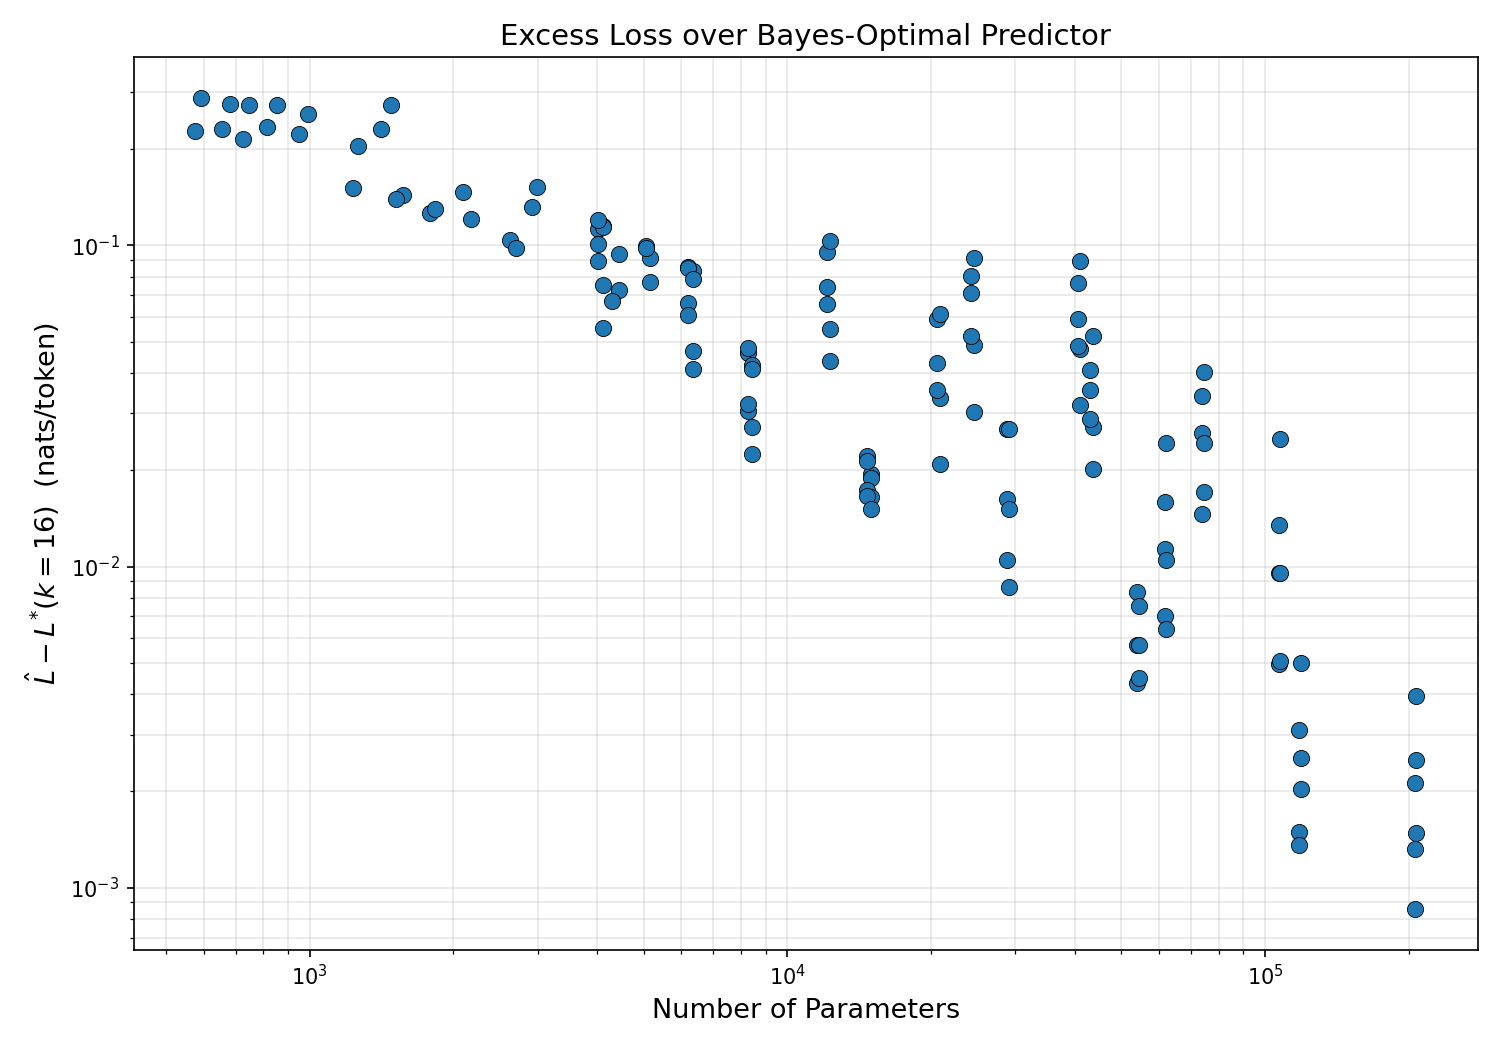
\includegraphics[width=\textwidth]{excess_loss_loglog.png}
    \caption{Excess loss $\hat{L} - L^{*}(k{=}16)$ on a log--log scale.  All architectural distinctions are suppressed to highlight the overall scaling trend with model size.}
    \label{fig:model-comparison-excess}
  \end{subfigure}
  \caption{Model size versus validation loss for 135 transformer configurations on the cylinder graph HMM\@.  (a)~Absolute validation loss.  (b)~Excess loss over the Bayes-optimal predictor at context length~$k = 16$.}
  \label{fig:model-comparison}
\end{figure}

Validation loss decreases roughly log-linearly with parameter count up to ${\sim}10^5$ parameters, after which gains diminish.  At every scale, full transformers (with MLP layers) outperform their attention-only counterparts, and all top-10 models use $L = 4$ layers.  LayerNorm has a negligible effect compared to architecture and scale.  The best model (L4, $d{=}64$, $H{=}4$, full, no-LN; ${\sim}206$k parameters) reaches ${\approx}\,2.473$\,nats/token.  By the decomposition in Eq.~\eqref{eq:loss-decomp}, most of the $0.034$\,nat gap above the entropy rate is attributable to the finite context window ($\Delta(16) \approx 0.03$\,nats), leaving only ${\sim}0.004$\,nats of model capacity gap.

\subsection{$N$-gram comparison}

Table~\ref{tab:ngram} reports the training and test cross-entropy loss for $n$-gram orders 1 through 6 (without regularisation; see Appendix~\ref{app:ngram-details} for smoothed results).

\begin{table}[htbp]
  \centering
  \begin{tabular}{r r r r}
    \toprule
    $n$ & Train CE & Test CE & \# Contexts \\
    \midrule
    1 & 3.654 & 3.652 &           1 \\
    2 & 2.667 & 2.669 &          48 \\
    3 & 2.551 & 2.566 &       1\,540 \\
    4 & 2.470 & 2.832 &      39\,531 \\
    5 & 2.236 & 4.781 &     443\,415 \\
    6 & 1.713 & 8.618 &   1\,953\,864 \\
    \bottomrule
  \end{tabular}
  \caption{$N$-gram cross-entropy (nats/token) without regularisation.  For $n \geq 4$, test loss diverges due to overfitting.  The best test performance is the trigram ($n = 3$).}
  \label{tab:ngram}
\end{table}

The largest drop in cross-entropy occurs from the unigram to the bigram ($3.65 \to 2.67$ nats), reflecting the strong first-order correlations induced by the HMM's clustered emission structure: observing a single token already reveals the current depth level, narrowing the effective vocabulary from~48 to~16.  The trigram provides a modest further gain, approaching the Bayes-optimal loss.  The best $n$-gram model (trigram, test CE $= 2.57$) is outperformed by transformers with embedding dimension $d \ge 16$, suggesting that these models learn to approximate belief-state inference beyond simple token co-occurrence statistics.  Conversely, very small transformers ($d = 4$) fail to beat the trigram, indicating that a minimum model capacity is needed before the transformer can surpass what a count table captures directly.

\subsection{Embedding structure}

Figure~\ref{fig:embedding} shows the cosine-similarity matrix and $\ell_2$ norms of the learned token-embedding vectors from a representative model.  The $3 \times 3$ block structure in the similarity matrix directly mirrors the depth-level clustering of the vocabulary: tokens within the same depth cluster are mapped to similar embedding directions, while cross-cluster pairs are near-orthogonal or anti-correlated.  This confirms that the model discovers the latent depth structure without supervision.

\begin{figure}[htbp]
  \centering
  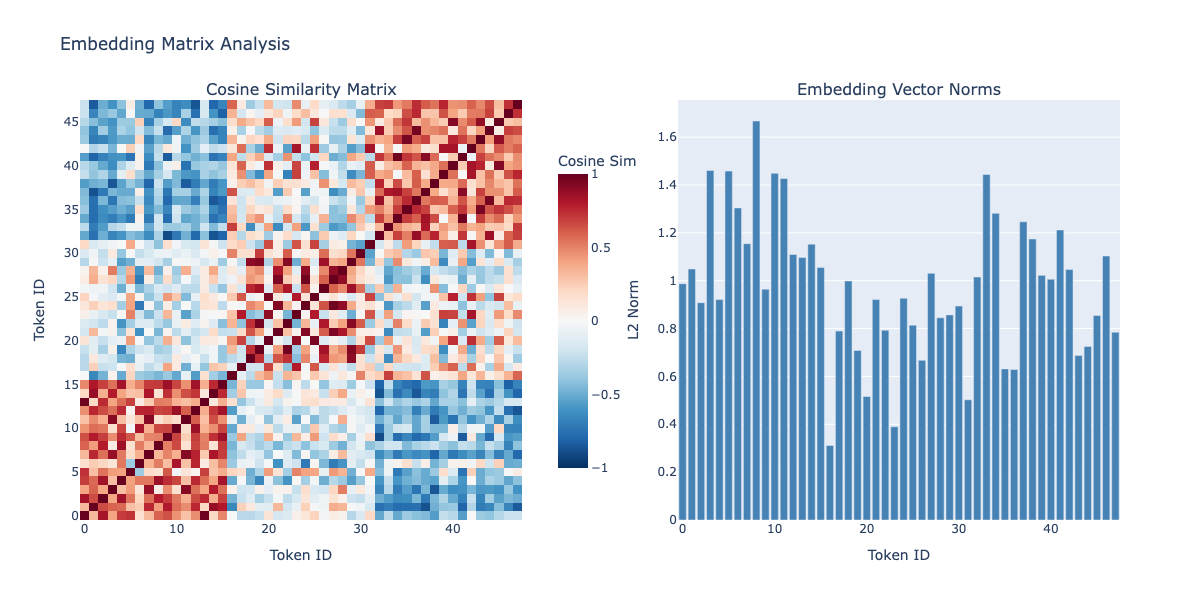
\includegraphics[width=0.85\textwidth]{newplot.png}
  \caption{Left: cosine similarity matrix of the $48 \times d$ embedding matrix.  The visible $3 \times 3$ block structure corresponds to the three depth levels.  Right: $\ell_2$ norm of each token's embedding vector.}
  \label{fig:embedding}
\end{figure}

\paragraph{Cluster similarity across architectures}
To quantify how consistently the embedding geometry reflects the depth-level structure, we compute the cosine similarity between cluster centroids across all 135 trained models.  For each model we extract the embedding matrix $W_E \in \mathbb{R}^{48 \times d}$ and compute three centroids
\begin{equation}
  \mathbf{c}_l = \frac{1}{16}\sum_{v=16l}^{16l+15} W_E[v,:],
  \qquad l \in \{0,1,2\},
\end{equation}
followed by the three pairwise cosine similarities $\mathrm{sim}(\mathbf{c}_0, \mathbf{c}_1)$, $\mathrm{sim}(\mathbf{c}_0, \mathbf{c}_2)$, and $\mathrm{sim}(\mathbf{c}_1, \mathbf{c}_2)$.

Figure~\ref{fig:cluster-sim} shows these similarities as a function of validation loss.  All three pairs are predominantly negative (mean $\approx -0.4$), confirming that the learned embeddings separate the three depth clusters into roughly opposing directions in embedding space.  Models that achieve low validation loss (left side of the plot) cluster tightly in the range $-0.35$ to $-0.50$, while poorly performing models exhibit much higher variance---some cluster pairs even become positively correlated.  This suggests that learning to separate the depth clusters in embedding space is necessary for good predictive performance, but the degree of separation saturates once the model is sufficiently expressive.

\begin{figure}[htbp]
  \centering
  \begin{subfigure}[t]{0.48\textwidth}
    \centering
    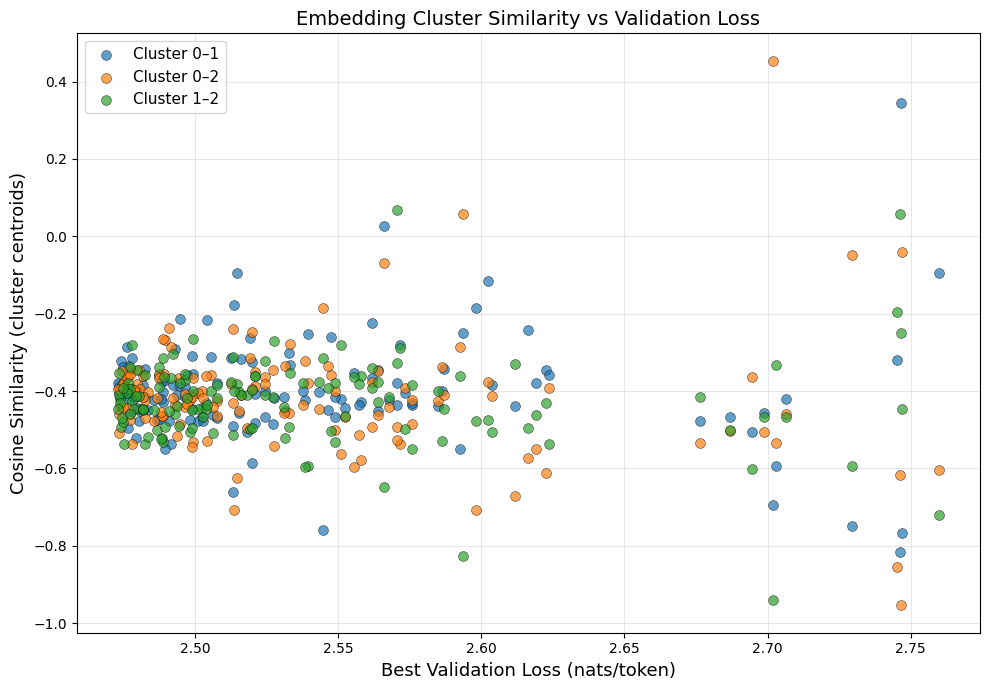
\includegraphics[width=\textwidth]{figures/embedding_cluster_similarity_raw.png}
    \caption{All three pairwise cosine similarities between cluster centroids, plotted for each of the 135 trained models.  Poorly performing models show high variance, with some cluster pairs becoming positively correlated.}
    \label{fig:cluster-sim-raw}
  \end{subfigure}
  \hfill
  \begin{subfigure}[t]{0.48\textwidth}
    \centering
    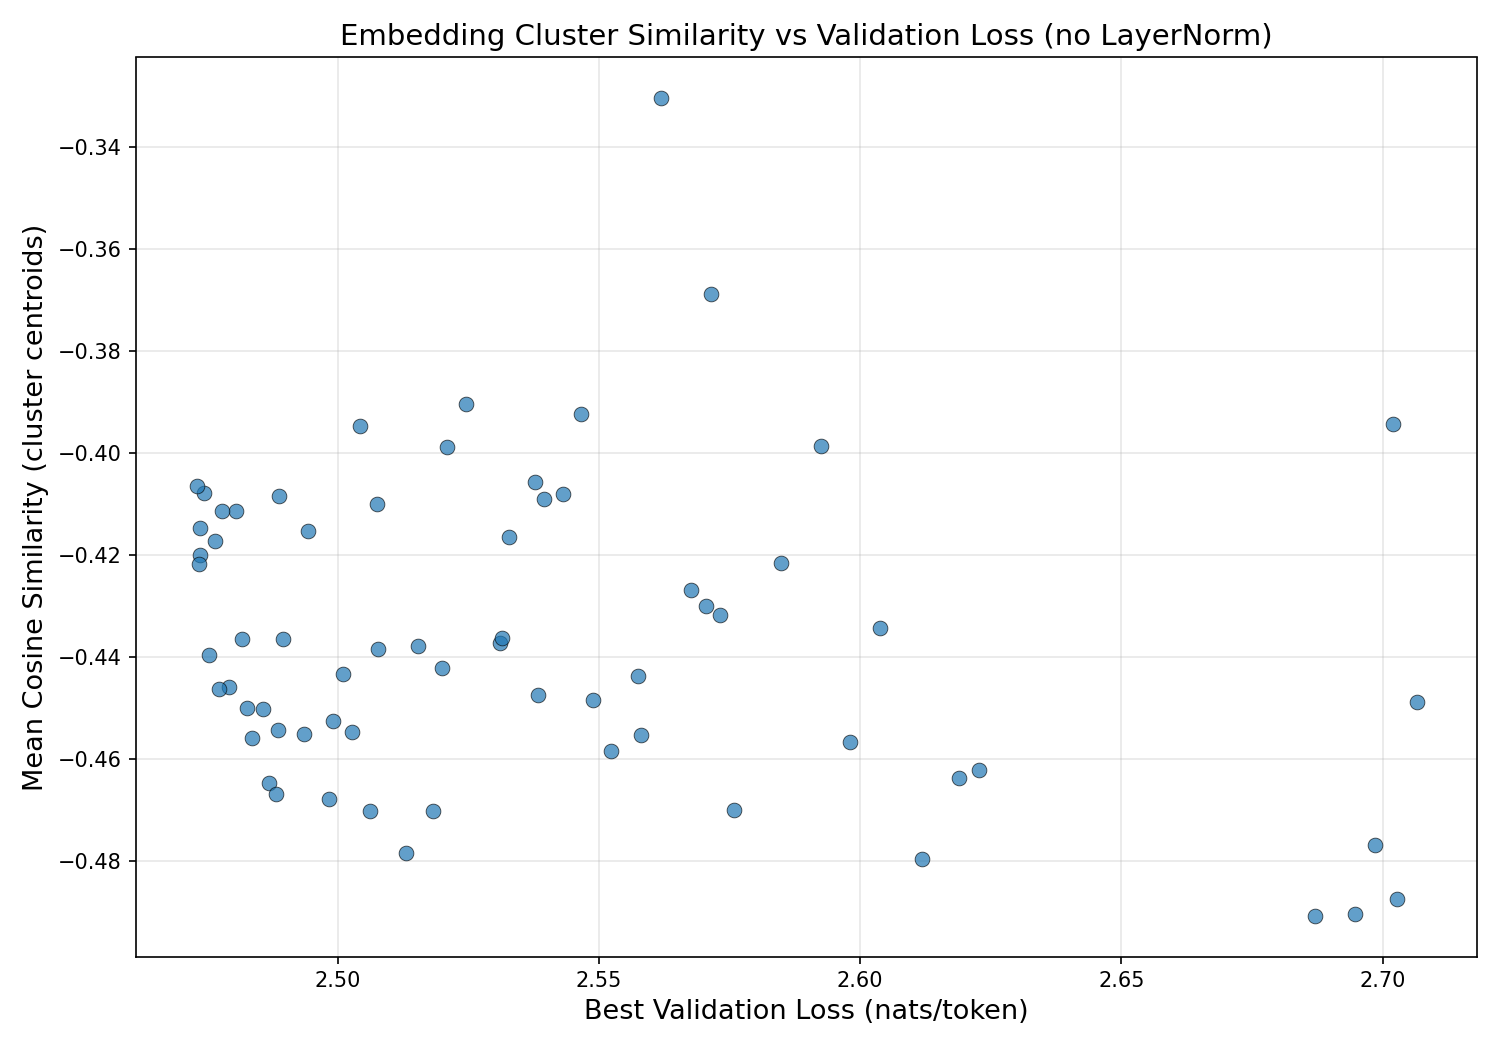
\includegraphics[width=\textwidth]{figures/embedding_cluster_similarity.png}
    \caption{Mean of the three pairwise similarities per model, restricted to architectures without LayerNorm (67~models).  The trend is flat, with most models in $[-0.49, -0.35]$.}
    \label{fig:cluster-sim-mean}
  \end{subfigure}
  \caption{Cosine similarity between depth-cluster centroids of the embedding matrix versus best validation loss.  (a)~Per-pair similarities for all models.  (b)~Mean similarity for noLN models only.}
  \label{fig:cluster-sim}
\end{figure}

%----------------------------------------------------------------------
\section{Summary and Open Questions}\label{sec:summary}
%----------------------------------------------------------------------

The cylinder graph HMM provides a controlled testbed for studying how transformers learn to perform approximate Bayesian filtering over a structured latent space.  Larger, deeper, full-architecture models approach but do not reach the entropy rate, suggesting fundamental limits tied to the autoregressive architecture and finite context.

Open directions include:
\begin{itemize}
  \item Characterising the belief-state geometry learned by the residual stream (cf.\ the fractal attractor structure discussed in Section~\ref{sec:geometry} and~\cite{shai2024}).
  \item Ablation studies on context length to quantify the loss attributable to finite $T$.
  \item Mechanistic interpretability of attention heads---do specific heads specialise in tracking depth transitions versus intra-layer dynamics?
\end{itemize}


%======================================================================
\appendix
%======================================================================

\section{$N$-gram Backoff Details}\label{app:ngram-details}

\paragraph{Backoff}
When an $(n{-}1)$-gram context has never been observed in training, the smoothed estimate degenerates to $1/|V|$.  To avoid this, we employ a simple backoff strategy: if the full $(n{-}1)$-gram context is absent from the count table, we fall back to the $(n{-}2)$-gram model, then the $(n{-}3)$-gram, and so on down to the unigram.  The first context length that appears in the training counts is used with its smoothed estimate.

%----------------------------------------------------------------------
\begin{thebibliography}{9}

\bibitem{baum1966}
L.~E. Baum and T.~Petrie,
``Statistical Inference for Probabilistic Functions of Finite State
Markov Chains,''
\emph{Annals of Mathematical Statistics}, 37(6):1554--1563, 1966.

\bibitem{rabiner1989}
L.~R. Rabiner,
``A Tutorial on Hidden Markov Models and Selected Applications in
Speech Recognition,''
\emph{Proceedings of the IEEE}, 77(2):257--286, 1989.

\bibitem{vaswani2017}
A.~Vaswani, N.~Shazeer, N.~Parmar, J.~Uszkoreit, L.~Jones,
A.~N. Gomez, \L.~Kaiser, and I.~Polosukhin,
``Attention Is All You Need,''
\emph{Advances in Neural Information Processing Systems}, 30, 2017.

\bibitem{rabiner1986}
L.~R. Rabiner and B.-H. Juang,
``An Introduction to Hidden Markov Models,''
\emph{IEEE ASSP Magazine}, 3(1):4--16, 1986.

\bibitem{shai2024}
A.~S. Shai, S.~E. Marzen, L.~Teixeira, A.~Gietelink Oldenziel,
and P.~M. Riechers,
``Transformers Represent Belief State Geometry in Their Residual Stream,''
in \emph{Advances in Neural Information Processing Systems~37 (NeurIPS)}, 2024.
\texttt{arXiv:2405.15943}.

\end{thebibliography}

\end{document}
